\documentclass[12pt]{beamer}
\usetheme{moloch}

\usepackage{amsmath,amscd}
\usepackage{fontspec}
\usepackage{unicode-math}
\usepackage[dvipsnames]{xcolor}
\usepackage{tikz}
\usepackage{pgfplots}
\pgfplotsset{compat=1.18}
\usetikzlibrary{positioning}
\usepackage{booktabs}
\usepackage{array}

\setbeamercolor{background canvas}{bg=black}
\setbeamercolor{normal text}{fg=white}

\setmonofont{DejaVu Sans Mono}

% Set the title bar to black background with white text
\setbeamercolor{frametitle}{bg=black, fg=white}

% Ensure other structural elements (bullets, etc.) are visible
\setbeamercolor{structure}{fg=white}

\iffalse
%\usepackage{ebgaramond}
\setmainfont{texgyrepagella}[
  Extension = .otf,
  UprightFont = *-regular,
  BoldFont = *-bold,
  ItalicFont = *-italic,
  BoldItalicFont = *-bolditalic,
  Color=charcoal,
]
\setmathfont{texgyrepagella-math.otf}
\fi

\iftrue
\setmainfont{Libertinus Serif}
\setsansfont{Libertinus Sans}
\setmonofont{DejaVu Sans Mono}
\setmathfont{STIXTwoMath-Regular.otf}
\fi

% Define colors for syntax highlighting
\definecolor{codegreen}{rgb}{0,0.6,0}
\definecolor{codegray}{rgb}{0.5,0.5,0.5}
\definecolor{codecoffee}{rgb}{0.75,0.6,0.3}
\definecolor{question}{rgb}{1.0,0.75,0.1}
\definecolor{lightblue}{rgb}{0.55,0.75,0.9}
\definecolor{yellow}{rgb}{1.0, 1.0, 0.0}
\definecolor{codecomment}{rgb}{0.97, 0.74, 0.4}
\definecolor{codepy}{rgb}{0.9, 0.85, 0.85} %{#F8BC65}
\definecolor{funcColor}{rgb}{0.47, 0.6, 0.8}
\definecolor{midgray}{rgb}{0.4, 0.4, 0.3}
\definecolor{indexwhite}{rgb}{0.9, 0.9, 0.9}

\newcommand{\FrameTitle}[2]{\frametitle{#1 \hfill \small\textnormal{\textcolor{midgray}{#2}}}}
\newcommand{\snl}{\vspace*{4pt}\\}
\newcommand{\nl}{\vspace*{1em}\\}
\newcommand{\vsp}{\vspace*{1em}}
\newcommand{\SixPtVspace}{\vspace*{6pt}}

\newcommand{\Quiz}[1]{{\large\textbf{\color{question}{#1}}}}
\newcommand{\QuizQuestion}[1]{{\Large\textbf{\color{question}{#1}}}}

\newcommand{\Matrix}[1]{\textbf{#1}}
\newcommand{\Vector}[1]{\textbf{#1}}
\newcommand{\MMat}[1]{\mathbf{#1}}
\newcommand{\MVec}[1]{\mathbf{#1}}
\newcommand{\Norm}[1]{\lVert {\mathbf{#1}} \rVert}
\newcommand{\NormBeta}[1]{\lVert \beta \mathbf{#1} \rVert}
\newcommand{\NormConst}[1]{\lVert #1 \rVert}
\newcommand{\Trans}{\text{\raisebox{0.5ex}{\scalebox{0.75}{T}}}}
\newcommand{\abs}[1]{\lvert {#1} \rvert}
\newcommand{\Avg}[1]{\mathbf{avg}(\mathbf{#1})}
\newcommand{\Std}[1]{\mathbf{std}(\mathbf{#1})}

\begin{document}
\title{\center{Applied Linear Algebra\\\vsp Matrix Calculus for Learning Systems\vspace*{4pt}\\Unit 3\\}}
\author{\center{Devi Prasad M \\ Manipal School of Information Sciences \\ Manipal \\}}
\date{\center{October 2026}}
\maketitle

\begin{frame}\FrameTitle{Topics and Time Allocation}{Unit 3}
    %\vspace*{-1em}
    \begin{itemize}
        \item Derivatives in one dimension \hfill (0.5 h)%
        \item Gradients in multiple dimensions \hfill (1 h)%
        \item Chain rule in multiple dimensions \hfill (1 h)%
        \item Gradients of matrix expressions \hfill (2 h)%
        \item Optimization using gradient descent \hfill(3.5 h)%
        \begin{itemize}
            \item single-sample updates
            \item Logistic regression (No hidden layer)
            \item Softmax regression (No hidden layer)
        \end{itemize}
        \item Backpropagation \hfill (3 h)%
        \begin{itemize}
            \item Computational graphs
            \item Multi-layer perceptrons (Hidden Layers)
        \end{itemize}
    \end{itemize}
\end{frame}

\begin{frame}\FrameTitle{Derivatives in One Dimension}{Unit 3}
    A derivative is the rate of change of a function with
    respect to changes in its inputs.

    \vsp
    For functions $f \, : \, \mathbb{R} \to \mathbb{R}$,
    the derivative of $f$ at $x$ is defined as:
              $$f'(x) = \lim_{h \to 0} \dfrac{f(x+h)-f(x)}{h}$$
\end{frame}

\begin{frame}\FrameTitle{Derivative - Rate of Change}{Unit 3}
    $f'(x)$ measures how fast the output changes as the
    input changes:
              $$f'(x) = \lim_{h \to 0} \dfrac{f(x+h)-f(x)}{h}$$

    \vsp
    This limit tells us what the ratio between the perturbation $h$
    in the input and the change in the function value $f(x+h)-f(x)$
    converges to as $h$ shrinks to zero.

    \vsp
    If the limit exists, we say that $f$ is \emph{differentiable} at $x$.
\end{frame}

\begin{frame}\FrameTitle{Derivatives in One Dimension}{Unit 3}
    \begin{itemize}
        \item \textbf{Local linearity.} Near any point, a smooth function
              behaves like a straight line:
              $$f(x+\Delta x) \approx f(x) + f'(x)\,\Delta x$$
        \item \textbf{Direction of descent.} To decrease $f$, move $x$ against
              the sign of $f'(x)$.
        \item At a minimum $f'(x)=0$, though not every
              point with $f'(x)=0$ is a minimum.
    \end{itemize}
\end{frame}

\begin{frame}\FrameTitle{The Chain Rule}{Unit 3}
    Rates of change multiply through a composition:
    \[
        \dfrac{d}{dx}\,f(g(x)) = f'(g(x))\,g'(x)
    \]

    \textbf{Follow a small nudge.} Write $y = g(x)$ and $z = f(y)$.
    \begin{center}
    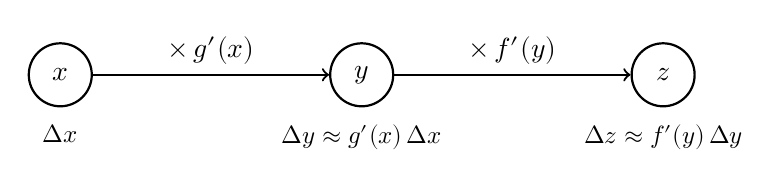
\begin{tikzpicture}[
        var/.style = {circle, draw, thick, minimum size=8mm, inner sep=0pt},
        node distance = 30mm
    ]
        \node[var]             (x) {$x$};
        \node[var, right=of x] (y) {$y$};
        \node[var, right=of y] (z) {$z$};
        \draw[->, thick] (x) -- node[above]{$\times\, g'(x)$}    (y);
        \draw[->, thick] (y) -- node[above]{$\times\, f'(y)$}    (z);
        \node[below=1mm of x] {\small $\Delta x$};
        \node[below=1mm of y] {\small $\Delta y \approx g'(x)\,\Delta x$};
        \node[below=1mm of z] {\small $\Delta z \approx f'(y)\,\Delta y$};
    \end{tikzpicture}
    \end{center}
    Substituting, $\Delta z \approx f'(y)\,g'(x)\,\Delta x$, so each stage
    scales the nudge and the scale factors multiply.

    \medskip
    \textbf{Example.} If $y$ changes $3\times$ as fast as $x$, and $z$ changes
    $2\times$ as fast as $y$, then $z$ changes $3 \times 2 = 6\times$ as fast as $x$.

    \medskip
    {\scriptsize\color{question}\textbf{Watch out.}
        $f'$ is evaluated at $y = g(x)$, where the nudge
        actually arrives, not at $x$.}

    \vfill
\end{frame}


% ---------------------------------------------------------------
\definecolor{hypblue}{RGB}{110,180,255}
\definecolor{hyporange}{RGB}{240,140,30}
\definecolor{hypgreen}{RGB}{40,170,90}

\begin{frame}\FrameTitle{The Chain Rule: Watching a Nudge Grow}{Unit 3}
    \textbf{Straight lines:} $y = 3x$, \ $z = 2y$. Nudge $x$ from $1$ to $1.1$.

    \begin{center}
    \begin{tikzpicture}[
        seg/.style  = {line width=3pt},
        tick/.style = {thick},
        lab/.style  = {below, font=\footnotesize},
        name/.style = {left, font=\small}
    ]
        % x line
        \draw[gray] (0,2.4) -- (6.4,2.4);
        \node[name] at (0,2.4) {$x$};
        \draw[seg, hypgreen] (0.6,2.4) -- (1.2,2.4);
        \draw[tick] (0.6,2.3) -- (0.6,2.5);  \node[lab] at (0.6,2.3) {$1$};
        \draw[tick] (1.2,2.3) -- (1.2,2.5);  \node[lab] at (1.25,2.3) {$1.1$};
        \node[right, font=\footnotesize, hypgreen] at (6.5,2.4) {$\Delta x = 0.1$};

        % y line
        \draw[gray] (0,1.2) -- (6.4,1.2);
        \node[name] at (0,1.2) {$y$};
        \draw[seg, hypblue] (0.6,1.2) -- (2.4,1.2);
        \draw[tick] (0.6,1.1) -- (0.6,1.3);  \node[lab] at (0.6,1.1) {$3$};
        \draw[tick] (2.4,1.1) -- (2.4,1.3);  \node[lab] at (2.4,1.1) {$3.3$};
        \node[right, font=\footnotesize, hypblue] at (6.5,1.2) {$\Delta y = 0.3$};

        % z line
        \draw[gray] (0,0) -- (6.4,0);
        \node[name] at (0,0) {$z$};
        \draw[seg, hyporange] (0.6,0) -- (4.2,0);
        \draw[tick] (0.6,-0.1) -- (0.6,0.1);  \node[lab] at (0.6,-0.1) {$6$};
        \draw[tick] (4.2,-0.1) -- (4.2,0.1);  \node[lab] at (4.2,-0.1) {$6.6$};
        \node[right, font=\footnotesize, hyporange] at (6.5,0) {$\Delta z = 0.6$};

        % stretch arrows
        \draw[->, thick] (3.2,2.25) -- node[right, font=\small]{$\times 3$} (3.2,1.4);
        \draw[->, thick] (5.0,1.05) -- node[right, font=\small]{$\times 2$} (5.0,0.2);
    \end{tikzpicture}
    \end{center}

    The derivative is the \textbf{stretch factor}:
    \[
        \frac{dy}{dx} = 3, \qquad \frac{dz}{dy} = 2, \qquad
        \frac{dz}{dx} = 3 \times 2 = 6.
    \]
    Check: $z = 2(3x) = 6x$.

    %\medskip
    %\textbf{On a curve,} the same picture holds, but only for small nudges
    %(next slide).
\end{frame}

\begin{frame}\FrameTitle{On Curves, the Chain Rule Holds Locally}{Unit 3}
    \vspace{-1em}
    {\small
    $y = x^3$, \ $z = y^2$, starting at $x = 1$. The derivatives predict
    \[
        \frac{dy}{dx} = 3x^2 = 3, \qquad
        \frac{dz}{dy} = 2y = 2, \qquad
        \frac{dz}{dx} = 3 \times 2 = 6.
    \]

    \vspace{-1mm}
    Now nudge $x$ by less and less:
    \begin{center}
    \scriptsize
    \begin{tabular}{l l c l c c}
        \toprule
        $\Delta x$ & $\Delta y$ & $\Delta y / \Delta x$ &
        $\Delta z$ & $\Delta z / \Delta y$ & $\Delta z / \Delta x$ \\
        \midrule
        $0.1$   & $0.331$     & $3.31$   & $0.7716$   & $2.331$  & $7.716$ \\
        $0.01$  & $0.030301$  & $3.0301$ & $0.061520$ & $2.0303$ & $6.152$ \\
        $0.001$ & $0.0030030$ & $3.0030$ & $0.0060150$ & $2.0030$ & $6.015$ \\
        \midrule
        $\to 0$ &             & $\to 3$  &            & $\to 2$  & $\to 6$ \\
        \bottomrule
    \end{tabular}
    \end{center}
    \small
    \begin{itemize}
        \item \textbf{Why not exactly $0.03$?} The slope predicts $0.03$;
              the extra $0.000301$ comes from the curve bending.
              Shrink the nudge $10\times$ and the extra shrinks $100\times$
              (to $0.000003$), so the slope's prediction takes over.
        \item In every row, $\tfrac{\Delta z}{\Delta x}
              = \tfrac{\Delta z}{\Delta y}\cdot\tfrac{\Delta y}{\Delta x}$
              exactly. As $\Delta x \to 0$, the factors become $3$ and $2$.
    \end{itemize}}
\end{frame}

%% {\tiny\color{lightblue}\url{https://www.3blue1brown.com/lessons/chain-rule-and-product-rule/}}%
\begin{frame}\FrameTitle{Functions in One Dimension}{Unit 3}
    \begin{columns}[t]
        \begin{column}{0.43\textwidth}
            \begin{block}{Basic Functions}
                \begin{itemize}
                    \item Exponential: $\exp(z)$\\\vspace*{1mm}
                        --- $e^{z}$
                    \item Natural Log: $\ln(z)$
                \end{itemize}
            \end{block}
        \end{column}

        \begin{column}{0.55\textwidth}
            \begin{block}{Activation Functions}
                \begin{itemize}
                    \item Sigmoid: $\sigma(z) = \dfrac{1}{1+e^{-z}}$
                    \item Tanh: $\tanh(z) = \dfrac{e^{z}-e^{-z}}{e^{z}+e^{-z}}$
                    \item ReLU: $\max(0,z)$
                    \item Leaky ReLU: $\max(0.01z,z)$
                    \item GELU: $z \cdot \Phi(z)$
                \end{itemize}
            \end{block}
        \end{column}
    \end{columns}
\end{frame}

% $\text{GELU}(z) \approx 0.5z \left(1 + \tanh\left(\sqrt{\frac{2}{\pi}} (z + 0.044715z^3)\right)\right)$

\begin{frame}\FrameTitle{Derivative of $e^z$}{Unit 3}
    \begin{align*}
        \frac{d}{dz}(e^z) &= \lim_{h \to 0} \dfrac{e^{z+h} - e^z}{h} \quad \text{(Limit definition)} \\[2pt]
        &= \lim_{h \to 0} \dfrac{e^z \cdot e^h - e^z}{h} \quad \text{(Exponent rules)} \\[2pt]
        &= \lim_{h \to 0} \dfrac{e^z(e^h - 1)}{h} \quad \text{(Factor out } e^z\text{)} \\[2pt]
        &= e^z \cdot \lim_{h \to 0} \dfrac{e^h - 1}{h} \quad \text{(Move } e^z \text{ outside the limit)} \\[2pt]
        &= e^z \cdot 1 \quad \text{(Using the identity } \lim_{h \to 0} \dfrac{e^h-1}{h} = 1\text{)} \\[2pt]
        &= e^z
    \end{align*}

    \vfill
    {\scriptsize\color{question}Python snippet to verify $e^h \approx 1 + h$ for small $h$.}
\end{frame}

\begin{frame}\FrameTitle{Derivative of the Natural Logarithm}{Unit 3}
    \begin{align*}
        \text{Let } y &= \ln(z) \\
            e^y &= z \quad \text{(Rewrite in exponential form)} \\[3pt]
            \frac{d}{dz}(e^y) &= \frac{d}{dz}(z) \quad \text{(Differentiate both sides)} \\[3pt]
            e^y \cdot \frac{dy}{dz} &= 1 \quad \text{(Apply the chain rule)}^{\dag} \\[3pt]
            \frac{dy}{dz} &= \frac{1}{e^y} \\[3pt]
            \frac{dy}{dz} &= \frac{1}{z} \quad \text{(Substitute } e^y = z \text{)}
    \end{align*}
    \vfill
    $\dag${\scriptsize\color{question}$f(g(z)) = e^{g(z)}, \ g(z) = y$.}
\end{frame}


\begin{frame}\FrameTitle{Derivative of the Sigmoid via the Chain Rule}{Unit 3}
    Simplify $\sigma(z) = 1/(1+e^{-z})$ into four steps.
    Operation is shown above the arrow, and the local derivative below the arrow.

    \begin{center}
    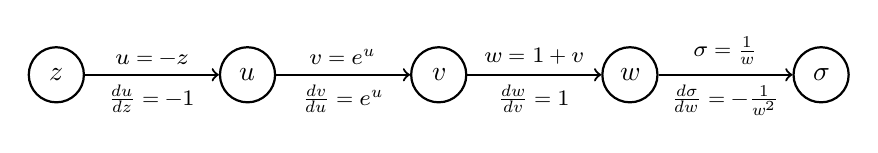
\begin{tikzpicture}[
        var/.style = {circle, draw, thick, minimum size=7mm, inner sep=0pt},
        op/.style  = {above, font=\footnotesize},
        loc/.style = {below, font=\footnotesize},
        node distance = 17mm
    ]
        \node[var]             (z) {$z$};
        \node[var, right=of z] (u) {$u$};
        \node[var, right=of u] (v) {$v$};
        \node[var, right=of v] (w) {$w$};
        \node[var, right=of w] (s) {$\sigma$};
        \draw[->, thick] (z) -- node[op]{$u=-z$}    node[loc]{$\frac{du}{dz}=-1$}    (u);
        \draw[->, thick] (u) -- node[op]{$v=e^{u}$} node[loc]{$\frac{dv}{du}=e^{u}$} (v);
        \draw[->, thick] (v) -- node[op]{$w=1+v$}   node[loc]{$\frac{dw}{dv}=1$}     (w);
        \draw[->, thick] (w) -- node[op]{$\sigma=\frac{1}{w}$}
                                node[loc]{$\frac{d\sigma}{dw}=-\frac{1}{w^{2}}$}     (s);
    \end{tikzpicture}
    \end{center}

    \textbf{Chain rule:} multiply the local derivatives along the chain.
    \[
        \frac{d\sigma}{dz}
        = \frac{d\sigma}{dw}\,\frac{dw}{dv}\,\frac{dv}{du}\,\frac{du}{dz}
        = \Bigl(-\frac{1}{w^{2}}\Bigr)(1)\,(e^{u})\,(-1)
        = \frac{e^{-z}}{(1+e^{-z})^{2}}
    \]

    \textbf{Rewrite in terms of $\sigma$:}
    \[
        \frac{e^{-z}}{(1+e^{-z})^{2}}
        = \underbrace{\frac{1}{1+e^{-z}}}_{\sigma(z)}
          \cdot
          \underbrace{\frac{e^{-z}}{1+e^{-z}}}_{1-\sigma(z)}
        \quad\Longrightarrow\quad
        \boxed{\sigma'(z) = \sigma(z)\bigl(1-\sigma(z)\bigr)}
    \]
\end{frame}

\begin{frame}\FrameTitle{More About the Sigmoid}{Unit 3}
    Show that $\sigma(-z) = 1 - \sigma(z)$

    \begin{align*}
        \textbf{Note} \ \sigma(z) &= \frac{1}{1+e^{-z}} \quad \textbf{and} \quad \sigma(-z) = \frac{1}{1+e^{z}} \\[2mm]
        1 - \sigma(z) &= 1 - \frac{1}{1+e^{-z}} \\[2mm]
                &= \frac{e^{-z}}{1+e^{-z}} \ = \ \frac{1}{e^{z}} \cdot \frac{1}{1+e^{-z}} \\[2mm]
                &= \frac{1}{1+e^{z}} \\[2mm]
                &= \sigma(-z)
    \end{align*}
\end{frame}

\begin{frame}\FrameTitle{Derivative of $\sigma(-z)$}{Unit 3}
    \vspace*{-1em}
    \begin{align*}
        \frac{d}{dz}\sigma(-z) &= \frac{d}{dz}\bigl(1-\sigma(z)\bigr) \\[1mm]
        &= 0 - \sigma'(z) \\[1mm]
        &= -\,\sigma(z)\,\bigl(1-\sigma(z)\bigr)
    \end{align*}
    \begin{itemize}
        \item $\sigma'(-z)$: take $\sigma'$, then evaluate it at $-z$.
              \[
                  \sigma'(-z) = \sigma(-z)\bigl(1-\sigma(-z)\bigr) \;>\; 0
              \]
        \item $\tfrac{d}{dz}\,\sigma(-z)$: differentiate the composite
              with respect to $z$.
              \[
                  \frac{d}{dz}\,\sigma(-z) = -\,\sigma'(-z) \;<\; 0
              \]
    \end{itemize}
    \medskip
    The two differ by exactly the chain-rule factor $\tfrac{d}{dz}(-z) = -1$.
\end{frame}

\begin{frame}\FrameTitle{Derivative of $\sigma(-z)$ Using the Chain Rule}{Unit 3}
Simplify $\sigma(-z) = 1/(1+e^{z})$ into four steps.
    \begin{center}
    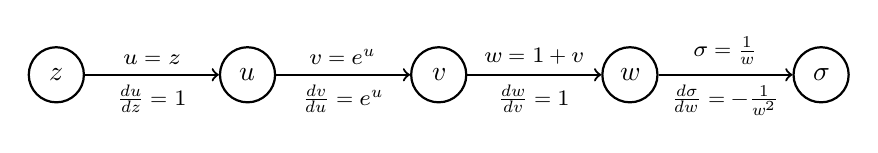
\begin{tikzpicture}[
        var/.style = {circle, draw, thick, minimum size=7mm, inner sep=0pt},
        op/.style  = {above, font=\footnotesize},
        loc/.style = {below, font=\footnotesize},
        node distance = 17mm
    ]
        \node[var]             (z) {$z$};
        \node[var, right=of z] (u) {$u$};
        \node[var, right=of u] (v) {$v$};
        \node[var, right=of v] (w) {$w$};
        \node[var, right=of w] (s) {$\sigma$};
        \draw[->, thick] (z) -- node[op]{$u=z$}    node[loc]{$\frac{du}{dz}=1$}    (u);
        \draw[->, thick] (u) -- node[op]{$v=e^{u}$} node[loc]{$\frac{dv}{du}=e^{u}$} (v);
        \draw[->, thick] (v) -- node[op]{$w=1+v$}   node[loc]{$\frac{dw}{dv}=1$}     (w);
        \draw[->, thick] (w) -- node[op]{$\sigma=\frac{1}{w}$}
                                node[loc]{$\frac{d\sigma}{dw}=-\frac{1}{w^{2}}$}     (s);
    \end{tikzpicture}
    \end{center}

    \textbf{Chain rule:} multiply the local derivatives along the chain.
    \[
        \frac{d\sigma}{dz}
        = \frac{d\sigma}{dw}\,\frac{dw}{dv}\,\frac{dv}{du}\,\frac{du}{dz}
        = \Bigl(-\frac{1}{w^{2}}\Bigr)(1)\,(e^{u})\,(1)
        = -\frac{e^{z}}{(1+e^{z})^{2}}
    \]

    \textbf{Rewrite in terms of $\sigma$:}
    {\small{\[
        -\frac{e^{z}}{(1+e^{z})^{2}}
        = -\underbrace{\frac{1}{1+e^{z}}}_{\sigma(-z)}
          \cdot
          \underbrace{\frac{e^{z}}{1+e^{z}}}_{1-\sigma(-z)}
        \quad\Longrightarrow\quad
        \boxed{\sigma'(-z) = -\sigma(-z)\bigl(1-\sigma(-z)\bigr)}
    \]}}
\end{frame}

\begin{frame}\FrameTitle{Derivative of $\sigma(-z)$ --- One More Time!}{Unit 3}
    Show the two forms of $\dfrac{d}{dz}\sigma(-z)$ are equivalent:
    \begin{align*}
        \dfrac{d}{dz}\sigma(-z) &= -\,\sigma(z)\bigl(1-\sigma(z)\bigr) \\[1mm]
        &= -\,(1-\sigma(-z))\,\sigma(-z) \quad\text{(Use $\sigma(-z) = 1-\sigma(z)$)} \\[1mm]
        &= -\,\sigma(-z)\,\bigl(1-\sigma(-z)\bigr) \quad\text{(Rearrange)}
    \end{align*}
\end{frame}

\begin{frame}\FrameTitle{The Sigmoid and Its Derivative}{Unit 3}
    \begin{columns}[c]
        \begin{column}{0.47\textwidth}
            \begin{tikzpicture}
            \begin{axis}[
                width=\linewidth, height=0.9\linewidth, font=\tiny,
                xmin=-6, xmax=6, ymin=0, ymax=1.18,
                xtick={-6,-3,0,3,6},
                ytick={0,0.25,0.5,1},
                %yticklabels={$0$,$\tfrac14$,$\tfrac12$,$1$},
                yticklabels={$0$,$0.25$,$0.5$,$1$},
                xlabel={$z$}, axis lines=left,
                grid=major, grid style={gray}, % style={gray!20} %
                legend style={at={(0.02,0.98)}, anchor=west,
                    font=\tiny, draw=none, fill=none}, % fill=white %
                every axis plot/.append style={thick, samples=121, domain=-6:6}
            ]
                \addplot[lightblue]{1/(1+exp(-x))};
                \addlegendentry{$\sigma(z)$}
                \addplot[red, dashed] {exp(-x)/(1+exp(-x))^2};
                \addlegendentry{$\sigma'(z)$}
                \addplot[only marks, mark=*, mark size=1.8pt]
                    coordinates {(0,0.5) (0,0.25)};
            \end{axis}
            \end{tikzpicture}
        \end{column}
        \begin{column}{0.51\textwidth}
            \begin{itemize}
                \item \textbf{Range.} $0 < \sigma(z) < 1$ and
                      $\sigma(0) = \tfrac12$, so the output reads as a probability.
                \item \textbf{Increasing.} $\sigma'(z) > 0$ for every $z$.
                \item \textbf{Bounded slope.} $\sigma'(z) \le \tfrac14$, largest
                      at $z = 0$: $p(1-p)$ peaks at $p = \tfrac12$.
                \item \textbf{Symmetry.} $\sigma(-z) = 1-\sigma(z)$, so
                      $\sigma'(-z) = \sigma'(z)$.
                \item \textbf{Flat tails.} $\sigma'(z) \to 0$ as
                      $|z| \to \infty$.
            \end{itemize}
        \end{column}
    \end{columns}
\end{frame}

\begin{frame}\FrameTitle{Saturation: When the Gradient Vanishes}{Unit 3}
    \begin{columns}[c]
        \begin{column}{0.38\textwidth}
            \centering
            \begin{tabular}{rcc}
                \toprule
                $z$ & $\sigma(z)$ & $\sigma'(z)$ \\
                \midrule
                $0$  & $0.5$     & $0.25$ \\
                $2$  & $0.881$   & $0.105$ \\
                $4$  & $0.982$   & $0.018$ \\
                $6$  & $0.998$   & $0.0025$ \\
                $10$ & $0.99995$ & $0.000045$ \\
                \bottomrule
            \end{tabular}
        \end{column}
        \begin{column}{0.60\textwidth}
            \begin{itemize}
                \item \textbf{Saturation.} For large $|z|$ the output barely
                      moves, so any gradient that passes through $\sigma'$
                      is tiny and learning slows.
                \item \textbf{Deep networks.} Each sigmoid layer scales the
                      backward signal by $\sigma' \le \tfrac14$, so it can
                      shrink layer after layer.
            \end{itemize}
        \end{column}
    \end{columns}

    \bigskip
    \textbf{The loss decides.} For $p = \sigma(\symbf{w}^\top\symbf{x})$:
    \begin{itemize}
        \item Cross-entropy: $\nabla_{\symbf{w}}\ell = (p-y)\,\symbf{x}$.
              The $\sigma'$ factor cancels.
        \item Squared error: $\nabla_{\symbf{w}}\ell = (p-y)\,p(1-p)\,\symbf{x}$.
              Nearly zero when the model is confidently wrong.
    \end{itemize}
\end{frame}

% ---------------------------------------------------------
% Non-differentiable points
% ---------------------------------------------------------
\pgfplotsset{
    kink/.style = {
        width=0.34\textwidth, height=0.34\textwidth,
        axis lines=middle, ymin=-1.6, ymax=2.3,
        xtick={-1,1,2}, ytick={1,2},
        tick label style={font=\scriptsize},
        clip=true, enlargelimits=false,
    },
    curve/.style     = {very thick, yellow, samples=2},
    lefttan/.style   = {thick, dashed, orange!100!black, samples=2},
    righttan/.style  = {thick, dashed, green!100!black, samples=2},
    kinkpt/.style    = {only marks, mark=*, mark size=2pt, black},
}

\begin{frame}\FrameTitle{When Left and Right Slopes Disagree}{Unit 3}
    %\centering
    \begin{center}
    \footnotesize
    \begin{tabular}{@{}*{3}{>{\centering\arraybackslash}p{0.30\textwidth}}@{}}
        % |x| -------------------------------------------------------
        \begin{tikzpicture}
        \begin{axis}[kink, xmin=-2, xmax=2]
            \addplot[lefttan,  domain=0:2]  {-x};
            \addplot[righttan, domain=-2:0] {x};
            \addplot[curve,    domain=-2:0] {-x};
            \addplot[curve,    domain=0:2]  {x};
            \addplot[kinkpt] coordinates {(0,0)};
        \end{axis}
        \end{tikzpicture}
        &
        % ReLU ------------------------------------------------------
        \begin{tikzpicture}
        \begin{axis}[kink, xmin=-2, xmax=2]
            \addplot[lefttan,  domain=0:2]  {0};
            \addplot[righttan, domain=-2:0] {x};
            \addplot[curve,    domain=-2:0] {0};
            \addplot[curve,    domain=0:2]  {x};
            \addplot[kinkpt] coordinates {(0,0)};
        \end{axis}
        \end{tikzpicture}
        &
        % Hinge -----------------------------------------------------
        \begin{tikzpicture}
        \begin{axis}[kink, xmin=-1, xmax=3]
            \addplot[lefttan,  domain=1:3]  {1-x};
            \addplot[righttan, domain=-1:1] {0};
            \addplot[curve,    domain=-1:1] {1-x};
            \addplot[curve,    domain=1:3]  {0};
            \addplot[kinkpt] coordinates {(1,0)};
        \end{axis}
        \end{tikzpicture}
        \\[2pt]
        \textbf{Absolute value} & \textbf{ReLU} & \textbf{Hinge loss} \\
        $f(x) = |x|$ & $f(x) = \max(0, x)$ & $f(x) = \max(0, 1-x)$ \\
        kink at $x=0$ & kink at $x=0$ & kink at $x=1$ \\[2pt]
        \textcolor{orange!100!black}{$f'_-(0) = -1$} &
        \textcolor{orange!100!black}{$f'_-(0) = 0$}  &
        \textcolor{orange!100!black}{$f'_-(1) = -1$} \\
        \textcolor{green!100!black}{$f'_+(0) = +1$} &
        \textcolor{green!100!black}{$f'_+(0) = 1$}  &
        \textcolor{green!100!black}{$f'_+(1) = 0$}
    \end{tabular}
    \end{center}

    \vspace*{1em}
    \small
    Dashed lines continue each side's slope past the kink:
    {\color{orange!100!black}left slope} and {\color{green!100!black}right slope}.

    \vspace*{1em}
    Two different lines: no single tangent, $f'$ does not exist there.
\end{frame}



\definecolor{hypblue}{RGB}{66,133,244}
\definecolor{hyporange}{RGB}{240,140,30}
\definecolor{hypgreen}{RGB}{40,170,90}
\definecolor{hypred}{RGB}{225,70,70}

% ---------------------------------------------------------------
\begin{frame}\FrameTitle{From Circle to Hyperbola}{Unit 3}
    \begin{columns}[t]
        \begin{column}{0.48\textwidth}
            \centering
            \textbf{Circle} \; $x^2 + y^2 = 1$

            \medskip
            \begin{tikzpicture}[scale=1.05]
                \fill[hypblue!35] (0,0) -- (1,0) arc[start angle=0, end angle=51.6, radius=1] -- cycle;
                \draw[->, gray] (-1.3,0) -- (2.3,0) node[right] {\scriptsize $x$};
                \draw[->, gray] (0,-1.3) -- (0,1.5) node[above] {\scriptsize $y$};
                \draw[very thick, hypblue] (0,0) circle[radius=1];
                \draw[thick] (0,0) -- (51.6:1);
                \fill (51.6:1) circle[radius=1.6pt];
                \node[above right, font=\footnotesize] at (51.6:1) {$(\cos t,\ \sin t)$};
                \node[font=\tiny, color=black] at (0.65,0.25) {$\tfrac{t}{2}$};
            \end{tikzpicture}

            \medskip
            $\cos^2 t + \sin^2 t = 1$
        \end{column}
        \begin{column}{0.48\textwidth}
            \centering
            \textbf{Hyperbola} \; $x^2 - y^2 = 1$

            \medskip
            \begin{tikzpicture}[scale=1.05]
                \fill[hyporange!40] (0,0) -- plot[domain=0:0.9, variable=\s, samples=30]
                    ({cosh(\s)}, {sinh(\s)}) -- cycle;
                \draw[->, gray] (-0.3,0) -- (2.3,0) node[right] {\scriptsize $x$};
                \draw[->, gray] (0,-1.3) -- (0,1.5) node[above] {\scriptsize $y$};
                \draw[dashed, gray] (0,0) -- (1.4,1.4);
                \draw[dashed, gray] (0,0) -- (1.3,-1.3);
                \draw[very thick, hyporange] plot[domain=-1.08:1.17, variable=\s, samples=60]
                    ({cosh(\s)}, {sinh(\s)});
                \draw[thick] (0,0) -- ({cosh(0.9)}, {sinh(0.9)});
                \fill ({cosh(0.9)}, {sinh(0.9)}) circle[radius=1.6pt];
                \node[right, font=\footnotesize] at ({cosh(0.9)}, {sinh(0.9)}) {$(\cosh t,\ \sinh t)$};
                \node[font=\tiny, color=black] at (0.75,0.25) {$\tfrac{t}{2}$};
            \end{tikzpicture}

            \medskip
            $\cosh^2 t - \sinh^2 t = 1$
        \end{column}
    \end{columns}

    \bigskip
    Shaded area $= \tfrac{t}{2}$ in both pictures. The hyperbolic pair is built from exponentials:
    \[
        \cosh t = \frac{e^{t} + e^{-t}}{2},
        \qquad
        \sinh t = \frac{e^{t} - e^{-t}}{2}.
    \]
\end{frame}

% ---------------------------------------------------------------
\begin{frame}\FrameTitle{Derivatives Without Sign Flips}{Unit 3}
    Differentiate the definitions directly:
    \[
        \frac{d}{dt}\cosh t = \frac{e^{t} - e^{-t}}{2} = \sinh t,
        \qquad
        \frac{d}{dt}\sinh t = \frac{e^{t} + e^{-t}}{2} = \cosh t.
    \]

    \vspace*{-2mm}
    \begin{columns}[c]
        \begin{column}{0.42\textwidth}
            \begin{tikzpicture}
            \begin{axis}[
                width=\linewidth, height=0.9\linewidth, color=white!80!black,
                xmin=-2.5, xmax=2.5, ymin=-3.2, ymax=3.2,
                xtick={-2,-1,1,2}, ytick={-2,2},
                xlabel={$t$}, axis lines=middle,
                tick label style={font=\tiny},
                legend style={at={(0.5,-0.08)}, anchor=north,
                              font=\tiny, draw=none, fill=none},
                legend columns=-1,
                legend style={/tikz/every even column/.append style={column sep=4pt}},
                legend cell align=left,
                every axis plot/.append style={samples=81, domain=-2.5:2.5}
            ]
                \addplot[very thick, hyporange] {cosh(x)};
                \addlegendentry{$\cosh t$}
                \addplot[very thick, hypblue] {sinh(x)};
                \addlegendentry{$\sinh t$}
                \addplot[thick, dashed, white!60] {exp(x)/2};
                \addlegendentry{$\tfrac12 e^{t}$}
            \end{axis}
            \end{tikzpicture}
        \end{column}
        \begin{column}{0.57\textwidth}
            \small
            \begin{itemize}
                \item Trigonometry has a sign flip, $(\cos t)' = -\sin t$.
                      The hyperbolic pair has \textbf{none}.
                \item $e^{t} = \cosh t + \sinh t$: cosh is the
                      \textbf{even} part of $e^{t}$, sinh the \textbf{odd} part.
                \item For large $t$, both approach $\tfrac12 e^{t}$ (dashed).
                %\item A hanging chain takes the shape $y = a\cosh(x/a)$, the \emph{catenary}.%
            \end{itemize}
        \end{column}
    \end{columns}
\end{frame}

% ---------------------------------------------------------------
\begin{frame}\FrameTitle{tanh: A ``Better'' Sigmoid}{Unit 3}
    \vspace*{-1em}
    \[
        \tanh z = \frac{\sinh z}{\cosh z} = \frac{e^{z} - e^{-z}}{e^{z} + e^{-z}}
    \]
    \vspace*{-1em}
    \begin{columns}[c]
        \begin{column}{0.40\textwidth}
            \begin{tikzpicture}
            \begin{axis}[
                width=1.1\linewidth, height=1.1\linewidth,
                xmin=-4, xmax=4, ymin=-1.15, ymax=1.15,
                xtick={-4,-2,2,4}, ytick={-1,0.5,1},
                xlabel={$z$}, axis lines=middle,
                tick label style={font=\scriptsize},
                legend style={at={(0.5,-0.08)}, anchor=north,
                              font=\footnotesize, draw=none, fill=none},
                legend columns=-1,
                legend style={/tikz/every even column/.append style={column sep=4pt}},
                legend cell align=left,
                every axis plot/.append style={samples=81, domain=-4:4}
            ]
                \addplot[very thick, hypgreen] {tanh(x)};
                \addlegendentry{$\tanh z$}
                \addplot[very thick, hypblue, dashed] {1/(1+exp(-x))};
                \addlegendentry{$\sigma(z)$}
                % tangent lines at z = 0: slope 1 for tanh, slope 1/4 for sigma
                \addplot[thin, hypgreen, domain=-0.9:0.9, forget plot] {x};
                \addplot[thin, hypblue,  domain=-1.8:1.8, forget plot] {0.5 + x/4};
                \addplot[only marks, mark=*, mark size=1.6pt, forget plot]
                    coordinates {(0,0) (0,0.5)};
            \end{axis}
            \end{tikzpicture}
        \end{column}
        \begin{column}{0.67\textwidth}
            \small
            \begin{itemize}
                \item \textbf{Same S-shape:} $\tanh z = 2\,\sigma(2z) - 1$,
                      the sigmoid stretched to $(-1, 1)$.
                \item \textbf{Zero-centred:} $\tanh 0 = 0$, outputs of both
                      signs. $\sigma$ outputs are always positive.
                \item \textbf{Steeper:} slope at $0$ is $1$, versus
                      $\tfrac14$ for $\sigma$ (thin lines).
                \item \textbf{Still saturates:} flat for large $|z|$,
                      so gradients still vanish there.
            \end{itemize}
        \end{column}
    \end{columns}

    \medskip
    {\color{question}{\scriptsize Check: $2\sigma(2z) - 1 = \dfrac{1-e^{-2z}}{1+e^{-2z}}$;
    multiply top and bottom by $e^{z}$ to get $\tanh z$.}}
\end{frame}

\begin{frame}\FrameTitle{Recap: The Quotient Rule}{Unit 3}
    For $h(x) = \dfrac{f(x)}{g(x)}$, wherever $g(x) \neq 0$:
    \[
        h'(x) = \frac{f'(x)\,g(x) - f(x)\,g'(x)}{g(x)^2}
    \]
    \begin{itemize}
        \item The order matters: the term with $f'$ comes first.
        \item The denominator is the original denominator, squared.
    \end{itemize}

    \medskip
    \textbf{Example.} $h(x) = \dfrac{x}{1+x^2}$, with $f = x$, $g = 1 + x^2$:
    \[
        h'(x) = \frac{1\cdot(1+x^2) - x\cdot 2x}{(1+x^2)^2}
              = \frac{1 - x^2}{(1+x^2)^2}
    \]
\end{frame}

\begin{frame}\FrameTitle{Derivative of Hyperbolic Tangent}{Unit 3}
    \begin{align*}
        \frac{d}{dz}\tanh z &= \frac{d}{dz}\,\frac{\sinh z}{\cosh z}\\[3mm]
            &= \frac{\cosh z \cdot \cosh z - \sinh z \cdot \sinh z}{\cosh^2 z}
            \qquad \text{(quotient rule)} \\[3mm]
            &= \frac{\cosh^2 z}{\cosh^2 z} - \frac{\sinh^2 z}{\cosh^2 z} = 1 - \tanh^2 z
\end{align*}
%Since $\cosh^2 z - \sinh^2 z = 1$, this also equals $\dfrac{1}{\cosh^2 z}$.
\end{frame}

\begin{frame}\FrameTitle{Derivative of tanh using the Chain Rule}{Unit 3}
    Start from $\tanh z = 2\,\sigma(2z) - 1$ and break it into three steps.
    Above each arrow is the operation; below it, the local derivative.

    \begin{center}
    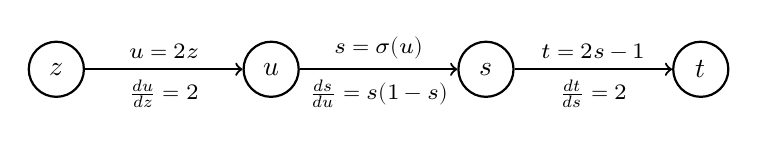
\begin{tikzpicture}[
        var/.style = {circle, draw, thick, minimum size=7mm, inner sep=0pt},
        op/.style  = {above, font=\footnotesize},
        loc/.style = {below, font=\footnotesize},
        node distance = 20mm
    ]
        \node[var]             (z) {$z$};
        \node[var, right=of z] (u) {$u$};
        \node[var, right=of u] (s) {$s$};
        \node[var, right=of s] (t) {$t$};
        \draw[->, thick] (z) -- node[op]{$u = 2z$}       node[loc]{$\frac{du}{dz} = 2$}                    (u);
        \draw[->, thick] (u) -- node[op]{$s = \sigma(u)$} node[loc]{$\frac{ds}{du} = s(1-s)$}               (s);
        \draw[->, thick] (s) -- node[op]{$t = 2s - 1$}   node[loc]{$\frac{dt}{ds} = 2$}                    (t);
    \end{tikzpicture}
    \end{center}

    \textbf{Chain rule:} multiply the local derivatives.
    \[
        \frac{d}{dz}\tanh z
        = \frac{dt}{ds}\,\frac{ds}{du}\,\frac{du}{dz}
        = 2 \cdot s(1-s) \cdot 2
        = 4\,\sigma(2z)\bigl(1-\sigma(2z)\bigr)
    \]

    \textbf{Rewrite in terms of tanh:} since $t = 2s - 1$,
    $s = \tfrac{1+\tanh z}{2}$ and $1-s = \tfrac{1-\tanh z}{2}$.
    \[
        4 \cdot \frac{1+\tanh z}{2} \cdot \frac{1-\tanh z}{2}
        = (1+\tanh z)(1-\tanh z)
        = \boxed{1 - \tanh^2 z}
    \]
\end{frame}

%% ---------------------------------------------------------------

%% Gradients in Multiple Dimensions
\begin{frame}\FrameTitle{Gradients in Multiple Dimensions}{Unit 3}
    \begin{itemize}
        \item \textbf{Partial derivative.} $\partial f/\partial x_j$: change one
              input, hold all the others fixed.
        \item \textbf{Gradient.} Collect the partials into a vector with the
              same shape as the input:
              $\nabla f(\symbf{x}) = \bigl[\partial f/\partial x_1, \dots,
              \partial f/\partial x_n\bigr]^\top$.
        \item \textbf{Local linearity.}
              $f(\symbf{x}+\Delta\symbf{x}) \approx f(\symbf{x})
              + \nabla f(\symbf{x})^\top \Delta\symbf{x}$.
        \item \textbf{Steepest ascent.} $\nabla f$ points in the direction of
              fastest increase and is perpendicular to the contour lines, so
              $-\nabla f$ is the steepest way downhill. At a minimum,
              $\nabla f = \symbf{0}$.
        \item \textbf{Jacobian.} For $\symbf{f}:\mathbb{R}^n \to \mathbb{R}^m$,
              the $m \times n$ matrix with entries
              $J_{ij} = \partial f_i/\partial x_j$ records how every output
              responds to every input.
    \end{itemize}
\end{frame}

\begin{frame}\FrameTitle{Chain Rule in Multiple Dimensions}{Unit 3}
    \begin{itemize}
        \item \textbf{Change flows through intermediate variables.} If
              $\symbf{x} \to \symbf{y} = \symbf{g}(\symbf{x}) \to z = f(\symbf{y})$,
              a change in $x_j$ reaches $z$ through every $y_i$ that depends
              on $x_j$.
        \item \textbf{Sum over paths.}
              $\displaystyle \dfrac{\partial z}{\partial x_j}
              = \sum_i \dfrac{\partial z}{\partial y_i}\,
                       \frac{\partial y_i}{\partial x_j}$:
              multiply along each path, then add across paths.
        \item \textbf{Matrix form.} Jacobians multiply:
              $\symbf{J}_{\symbf{f}\circ\symbf{g}}(\symbf{x})
              = \symbf{J}_{\symbf{f}}\bigl(\symbf{g}(\symbf{x})\bigr)\,
                \symbf{J}_{\symbf{g}}(\symbf{x})$.
        \item \textbf{Scalar output.} When the final output is one number
              (a loss),
              $\nabla_{\symbf{x}} z = \symbf{J}_{\symbf{g}}(\symbf{x})^\top
              \nabla_{\symbf{y}} z$: the gradient is passed backward through
              the transposed Jacobian.
    \end{itemize}
\end{frame}

\begin{frame}\FrameTitle{Gradients of Matrix Expressions}{Unit 3}
    \begin{itemize}
        \item \textbf{Shape rule.} The gradient of a scalar with respect to a
              vector or matrix has the same shape as that vector or matrix.
              Checking shapes catches most errors.
        \item \textbf{Method.} Write the expression with indices, differentiate
              a single entry, then reassemble the result in matrix form.
        \item \textbf{Standard results.}
              $\nabla_{\symbf{x}}(\symbf{a}^\top\symbf{x}) = \symbf{a}$, \;
              $\nabla_{\symbf{x}}(\symbf{x}^\top\symbf{A}\symbf{x})
                = (\symbf{A}+\symbf{A}^\top)\symbf{x}$, \;
              $\nabla_{\symbf{x}}\lVert\symbf{A}\symbf{x}-\symbf{b}\rVert^2
                = 2\symbf{A}^\top(\symbf{A}\symbf{x}-\symbf{b})$.
        \item \textbf{Linear layer.} For $\symbf{z} = \symbf{W}\symbf{x}$ and a
              scalar loss $L$:
              $\nabla_{\symbf{x}} L = \symbf{W}^\top \nabla_{\symbf{z}} L$ and
              $\nabla_{\symbf{W}} L = (\nabla_{\symbf{z}} L)\,\symbf{x}^\top$,
              an outer product.
        \item \textbf{Elementwise functions.} For
              $\symbf{h} = \phi(\symbf{z})$ applied entry by entry, the
              Jacobian is diagonal, so
              $\nabla_{\symbf{z}} L = \nabla_{\symbf{h}} L \odot \phi'(\symbf{z})$.
    \end{itemize}
\end{frame}


\begin{frame}\FrameTitle{Optimization Using Gradient Descent}{Unit 3}
    \begin{itemize}
        \item \textbf{Learning as minimization.} Training means choosing
              parameters $\symbf{\theta}$ that minimize the average loss
              $L(\symbf{\theta}) = \frac{1}{N}\sum_{n=1}^{N} \ell_n(\symbf{\theta})$.
        \item \textbf{Update rule.}
              $\symbf{\theta} \leftarrow \symbf{\theta} - \eta\,\nabla L(\symbf{\theta})$.
              By local linearity, a small step along $-\nabla L$ lowers the
              loss. If $\eta$ is too small, progress is slow; if too large,
              the steps overshoot or diverge.
        \item \textbf{Single-sample updates.}
              $\symbf{\theta} \leftarrow \symbf{\theta} - \eta\,\nabla \ell_n(\symbf{\theta})$
              for a randomly chosen example $n$. Each step is cheap, and the
              gradient is noisy but correct on average.
    \end{itemize}
\end{frame}

\begin{frame}\FrameTitle{Optimization Using Gradient Descent}{Unit 3}
    \begin{itemize}
        \item \textbf{Logistic regression.}
              $p = \sigma(\symbf{w}^\top\symbf{x} + b)$ with cross-entropy loss
              gives $\nabla_{\symbf{w}} \ell = (p - y)\,\symbf{x}$:
              prediction error times input.
        \item \textbf{Softmax regression.}
              $\symbf{p} = \operatorname{softmax}(\symbf{W}\symbf{x} + \symbf{b})$
              with cross-entropy loss gives
              $\nabla_{\symbf{W}} \ell = (\symbf{p} - \symbf{y})\,\symbf{x}^\top$
              for one-hot $\symbf{y}$, the same pattern extended to $K$ classes.
              Both losses are convex, so every local minimum is a global one.
    \end{itemize}
\end{frame}

\begin{frame}\FrameTitle{Backpropagation}{Unit 3}
    \begin{itemize}
        \item \textbf{Computational graph.} The model and loss are written as a
              chain of simple operations. Each node needs only its own local
              derivative.
        \item \textbf{Forward, then backward.} The forward pass computes and
              stores every intermediate value. The backward pass applies the
              chain rule from the loss toward the inputs, reusing those stored
              values.
        \item \textbf{Error signals.} Each node receives
              $\partial L/\partial(\text{node})$ from the nodes it feeds.
              When a value feeds several nodes, the incoming signals add.
        \item \textbf{Efficiency.} One backward pass gives the gradient for
              every parameter, at a cost comparable to one forward pass.
    \end{itemize}
\end{frame}

\begin{frame}\FrameTitle{Backpropagation}{Unit 3}
    \begin{itemize}
        \item \textbf{Multi-layer perceptron.} With
            $\symbf{z}_1 = \symbf{W}_1\symbf{x} + \symbf{b}_1$,
            $\symbf{h} = \phi(\symbf{z}_1)$,
            $\symbf{p} = \operatorname{softmax}(\symbf{W}_2\symbf{h} + \symbf{b}_2)$:
                $$\symbf{\delta}_2 = \symbf{p} - \symbf{y},$$
                $$\nabla_{\symbf{W}_2} L = \symbf{\delta}_2 \symbf{h}^\top,$$
                $$\symbf{\delta}_1 = (\symbf{W}_2^\top \symbf{\delta}_2) \odot \phi'(\symbf{z}_1),$$
                $$\nabla_{\symbf{W}_1} L = \symbf{\delta}_1 \symbf{x}^\top$$
        \item \textbf{Non-convexity.} Hidden layers make the loss non-convex.
              Gradient descent reaches a local solution, and that solution
              depends on the initialization.
    \end{itemize}
\end{frame}

\begin{frame}\FrameTitle{Reference Books}{Unit 3}
    \begin{itemize}
        \item Michael Nielsen, \emph{Neural Networks and Deep Learning}\\\vspace*{4pt}
            \href{http://neuralnetworksanddeeplearning.com/}{http://neuralnetworksanddeeplearning.com/}
        \vspace*{8pt}
        \item François Chollet, \emph{Deep Learning with Python},\\\vspace*{4pt}
            \href{https://www.manning.com/books/deep-learning-with-python}{https://www.manning.com/books/deep-learning-with-python}
        \item \href{https://www.3blue1brown.com/}{3Blue1Brown}\\\vspace*{4pt}
            \href{https://www.3blue1brown.com/?topic=calculus}{https://www.3blue1brown.com/?topic=calculus}
    \end{itemize}
\end{frame}
\end{document}
